

\def\layersep{2.5cm}
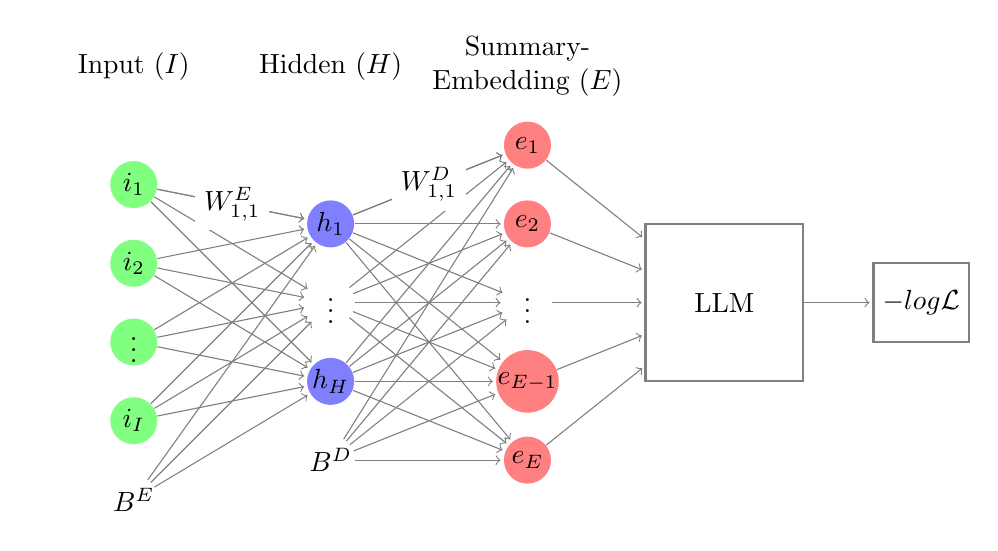
\begin{tikzpicture}[shorten >=1pt,->,draw=black!50, node distance=\layersep]
    \tikzstyle{every pin edge}=[<-,shorten <=1pt]
    \tikzstyle{neuron}=[circle,fill=black!25,minimum size=17pt,inner sep=0pt]
    \tikzstyle{LLM}=[draw,thick,minimum width=2cm, minimum height=2cm]
    \tikzstyle{NLL}=[draw,thick,minimum width=1cm, minimum height=1cm]
    \tikzstyle{bias neuron}=[neuron, fill=white];
    \tikzstyle{input neuron}=[neuron, fill=green!50];
    \tikzstyle{output neuron}=[neuron, fill=red!50];
    \tikzstyle{hidden neuron}=[neuron, fill=blue!50];
    \tikzstyle{annot} = [text width=7em, text centered]

    \node[input neuron] (I-1) at (0, -1) {$i_1$};
    \node[input neuron] (I-2) at (0, -2) {$i_2$};
    \node[input neuron] (I-3) at (0, -3) {$\vdots$};
    \node[input neuron] (I-4) at (0, -4) {$i_I$};
    \node[bias neuron] (I-5) at (0, -5) {$B^{E}$};

    \node[hidden neuron] (H-1) at (\layersep, -1.5) {$h_1$};
    \node[bias neuron] (H-2) at (\layersep, -2.5) {$\vdots$};
    \node[hidden neuron] (H-3) at (\layersep, -3.5) {$h_H$};
    \node[bias neuron] (H-4) at   (\layersep, -4.5) {$B^{D}$};

    \node[output neuron] (O-1) at (\layersep * 2, -0.5) {$e_1$};
    \node[output neuron] (O-2) at (\layersep * 2, -1.5) {$e_2$};
    \node[bias neuron] (O-3) at (\layersep * 2, -2.5) {$\vdots$};
    \node[output neuron] (O-4) at (\layersep * 2, -3.5) {$e_{E-1}$};
    \node[output neuron] (O-5) at (\layersep * 2, -4.5) {$e_E$};
    
    \node[LLM] (M-1) at (\layersep * 3, -2.5) {LLM};
    
    \node[NLL] (N-1) at (\layersep * 4, -2.5) {$- log \mathcal{L}$};

    \foreach \source in {1,...,5}
      \foreach \dest in {1,...,3}
        \path (I-\source) edge (H-\dest);
    
    \foreach \source in {1,...,4}
      \foreach \dest in {1,...,5}
        \path (H-\source) edge (O-\dest);

    \foreach \source in {1,...,5}
        \path (O-\source) edge (M-1);

    \draw (I-1) -- (H-1) node [midway, fill=white, minimum size=2pt] {$W_{1,1}^{E}$};
    \draw (H-1) -- (O-1) node [midway, fill=white, minimum size=2pt] {$W_{1,1}^{D}$};

    \path (M-1) edge (N-1);

    % Annotate the layers
    \node[annot,above of=H-1, node distance=2cm] (hl) {Hidden ($H$)};
    \node[annot,right of=hl] {Summary-Embedding ($E$)};
    \node[annot,left of=hl] {Input ($I$)};

\end{tikzpicture}